\apendice{Manual de usuario}
\label{apendice:manual_usuario}

\section{Introducción}
\label{sec:e-introduccion}

Este manual describe el uso práctico de la suite formada por dos add-ons para Blender. El primer add-on, \textit{Data Logger 3D}, permite registrar una sesión de modelado y exportar un CSV con los datos capturados. El segundo add-on permite leer esos CSV, calcular métricas estadísticas A1--A17, obtener métricas geométricas y UV, y generar visualizaciones dentro de Blender.

El contenido se ordena siguiendo el flujo real de trabajo: requisitos del sistema, instalación, configuración, uso del logger, exportación, uso del add-on de análisis, interpretación de métricas, diagnóstico de incidencias, privacidad y recomendaciones para organizar datos.

\section{Requisitos del sistema}
\label{sec:e-requisitos-sistema}

Para utilizar la suite se requiere una instalación funcional de Blender con soporte para add-ons de Python. El sistema debe permitir instalar scripts o paquetes ZIP desde el panel de preferencias. También se recomienda disponer de permisos de escritura en la carpeta del proyecto para poder exportar los CSV generados.

\begin{table}[H]
\centering
\scriptsize
\renewcommand{\arraystretch}{1.15}
\begin{tabularx}{\textwidth}{p{3.5cm}X}
\toprule
\textbf{Elemento} & \textbf{Requisito} \\
\midrule
Blender & Versión compatible con la API utilizada por los add-ons. Minimo 4.0.0. \\
Python & Python integrado en Blender. No se requiere ejecutar Python externo para el uso básico. \\
Add-on de captura & Archivo \texttt{DeteccionDatosV6.py}. \\
Add-on de análisis & Archivo ZIP del paquete de análisis. \\
Permisos de archivo & Escritura en la carpeta donde se guarda el \texttt{.blend} para exportar CSV. \\
Dependencias científicas & NumPy y Matplotlib si se utilizan las funciones analíticas y gráficas que las requieren. \\
\bottomrule
\end{tabularx}
\caption{Requisitos básicos para utilizar la suite.}
\label{tab:e-requisitos}
\end{table}

\section{Instalación y configuración}
\label{sec:e-instalacion}

La instalación de ambos add-ons se realiza desde el sistema estándar de Blender. Se recomienda instalar primero el logger y después el add-on de análisis.

\begin{enumerate}
    \item Abrir Blender.
    \item Acceder a \textit{Edit $\rightarrow$ Preferences $\rightarrow$ Add-ons}.
    \item Pulsar \textit{Install}.
    \item Seleccionar \texttt{DeteccionDatosV6.py} para instalar \textit{Data Logger 3D}.
    \item Activar la casilla del add-on instalado.
    \item Repetir el proceso con el ZIP del add-on de análisis.
    \item Guardar las preferencias si se desea conservar la activación en futuras sesiones.
\end{enumerate}

\begin{figure}[H]
    \centering
    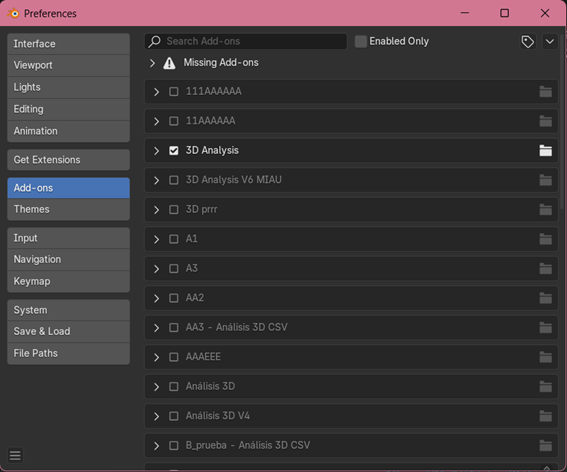
\includegraphics[width=0.85\textwidth]{diagramas/preferences.png}
    \caption{Ventana de preferencias de Blender para la instalación de add-ons.}
    \label{fig:e-preferences-addons}
\end{figure}

\begin{figure}[H]
    \centering
    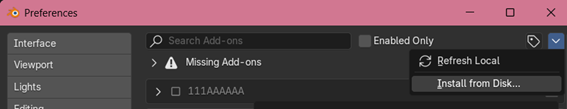
\includegraphics[width=0.85\textwidth]{diagramas/install.png}
    \caption{Botón de instalación de add-ons desde las preferencias de Blender.}
    \label{fig:e-install-addon}
\end{figure}

\begin{figure}[H]
    \centering
    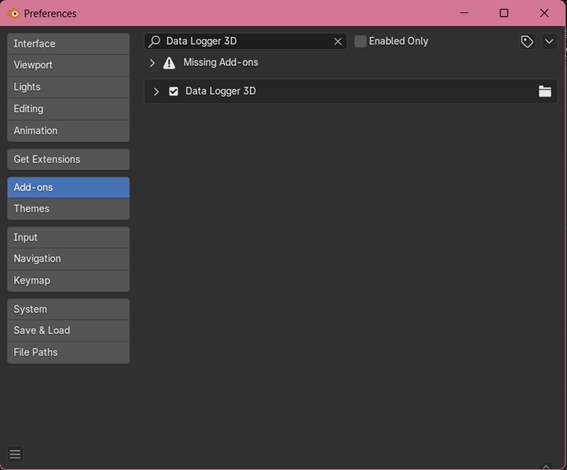
\includegraphics[width=0.85\textwidth]{diagramas/logger_activado.png}
    \caption{Add-on Data Logger 3D instalado y activado en Blender.}
    \label{fig:e-data-logger-activado}
\end{figure}

\begin{figure}[H]
    \centering
    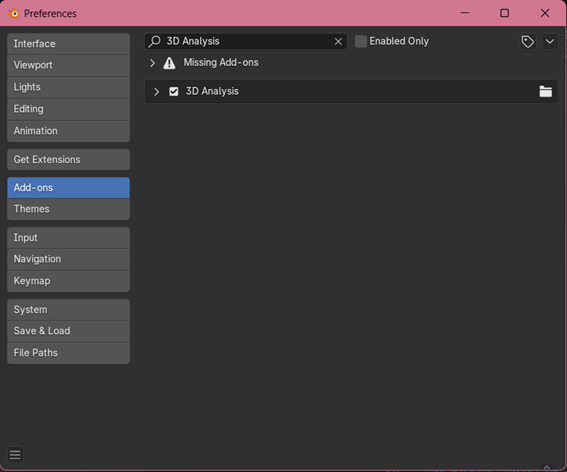
\includegraphics[width=0.85\textwidth]{diagramas/3D_analisys.png}
    \caption{Add-on de análisis y visualización instalado y activado en Blender.}
    \label{fig:e-addon-analisis-activado}
\end{figure}

\subsection{Configuración de Auto Run}
\label{subsec:e-autorun}

Si el archivo \texttt{.blend} necesita ejecutar scripts automáticamente al abrirse, Blender puede requerir que esté activada la opción Auto Run. Esta opción se encuentra en \textit{Edit $\rightarrow$ Preferences $\rightarrow$ File Paths $\rightarrow$ Auto Run Python Scripts}. Si Auto Run está desactivado, el logger muestra un aviso y no debe iniciarse la captura hasta que el usuario revise esta configuración.

\begin{figure}[H]
    \centering
    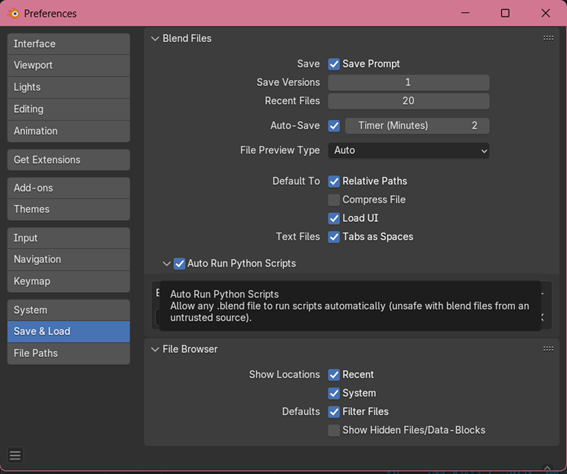
\includegraphics[width=0.85\textwidth]{diagramas/autorun.png}
    \caption{Configuración de Auto Run Python Scripts en las preferencias de Blender.}
    \label{fig:e-autorun}
\end{figure}

\section{Uso del Data Logger 3D}
\label{sec:e-uso-logger}

\subsection{Preparación de la sesión}
\label{subsec:e-preparacion-logger}

El funcionamiento previsto del add-on \textit{Data Logger 3D} se basa en la carga del archivo de Blender y en la aceptación explícita del consentimiento. Una vez instalado y activado el add-on, se recomienda guardar el archivo \texttt{.blend}, cerrar Blender y volver a abrir el proyecto. Al abrir de nuevo el archivo, el sistema muestra la ventana de consentimiento. Cuando el usuario acepta la recopilación de datos técnicos, el logger comienza la captura automáticamente.

Este flujo evita que el usuario tenga que iniciar manualmente la captura desde el panel en condiciones normales de uso. El panel del add-on permanece disponible para comprobar el estado del registro, detener la captura si fuera necesario y exportar posteriormente el archivo CSV generado.

\begin{enumerate}
    \item Abrir o crear el proyecto de modelado en Blender.
    \item Instalar y activar el add-on \textit{Data Logger 3D}.
    \item Guardar el archivo \texttt{.blend}.
    \item Cerrar Blender.
    \item Volver a abrir el archivo \texttt{.blend} guardado.
    \item Revisar la configuración de Auto Run si Blender muestra el aviso correspondiente.
    \item Aceptar la ventana de consentimiento de recopilación de datos técnicos.
    \item Comprobar en la pestaña \textit{Data Logger} que la captura se encuentra activa.
\end{enumerate}

\begin{figure}[H]
    \centering
    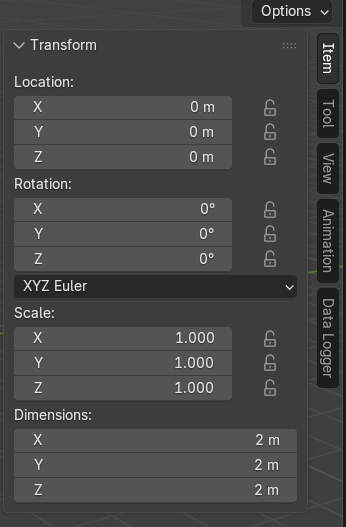
\includegraphics[width=0.85\textwidth]{diagramas/n.png}
    \caption{Ubicación de la pestaña Data Logger en la barra lateral del visor 3D.}
    \label{fig:e-sidebar-data-logger}
\end{figure}

\subsection{Consentimiento}
\label{subsec:e-consentimiento}

El sistema solicita consentimiento antes de registrar datos técnicos de la sesión. Esta ventana aparece al volver a abrir el archivo \texttt{.blend} después de haber instalado y activado el add-on. La captura no comienza hasta que el usuario acepta expresamente dicha recopilación.

Una vez aceptado el consentimiento, el add-on inicia automáticamente el registro de la sesión. El consentimiento se almacena en el propio archivo mediante un bloque interno, por lo que se recomienda guardar de nuevo el \texttt{.blend} después de aceptarlo. De esta forma, la aceptación puede conservarse junto al proyecto para sesiones posteriores.

Los datos capturados son técnicos: transformaciones, posición de vista, deltas topológicos, cambios UV, modificadores, modos y operadores relevantes. No se registran pulsaciones generales de teclado, contenido textual externo, conversaciones, credenciales ni datos personales directos.

\begin{figure}[H]
    \centering
    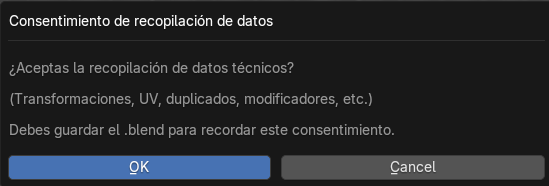
\includegraphics[width=0.65\textwidth]{diagramas/consentimiento.png}
    \caption{Ventana de consentimiento mostrada antes de iniciar la captura de datos técnicos.}
    \label{fig:e-consentimiento-logger}
\end{figure}

\subsection{Inicio automático y control manual de la captura}
\label{subsec:e-inicio-parada}

El inicio normal de la captura se produce automáticamente tras aceptar la ventana de consentimiento. En ese momento, el logger queda activo y comienza a registrar en segundo plano los cambios significativos de la sesión de modelado. Por tanto, en el flujo previsto no es necesario pulsar manualmente \textit{Start Logger} para comenzar la grabación.

El panel principal del logger muestra el estado de la captura y permite controlar manualmente el proceso cuando sea necesario. Si el logger está detenido, el botón \textit{Start Logger} permite iniciar el registro de forma manual. Si el logger está activo, el botón \textit{Stop Logger} permite detenerlo. Al detenerse, el CSV se incrusta en el archivo \texttt{.blend}, lo que permite conservar los datos junto al proyecto antes de exportarlos.

Este control manual resulta útil para comprobar el funcionamiento del add-on, reiniciar una captura o detener el registro antes de finalizar la sesión.

\begin{figure}[H]
    \centering
    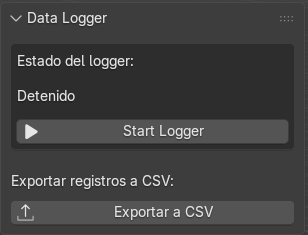
\includegraphics[width=0.65\textwidth]{diagramas/parado.png}
    \caption{Panel principal del Data Logger 3D antes de iniciar la captura.}
    \label{fig:e-panel-logger-detenido}
\end{figure}

\begin{figure}[H]
    \centering
    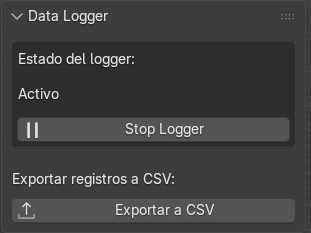
\includegraphics[width=0.65\textwidth]{diagramas/activo.png}
    \caption{Panel principal del Data Logger 3D durante una sesión de captura activa.}
    \label{fig:e-panel-logger-activo}
\end{figure}

\begin{figure}[H]
    \centering
    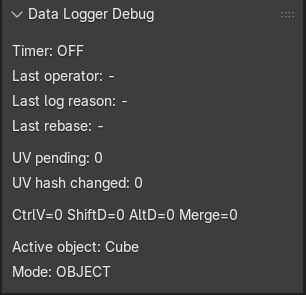
\includegraphics[width=0.65\textwidth]{diagramas/data_logger_con_debug.png}
    \caption{Panel de depuración del Data Logger 3D con información del último evento registrado.}
    \label{fig:e-panel-debug-logger}
\end{figure}

\subsection{Operaciones detectadas}
\label{subsec:e-operaciones-detectadas}

Durante la captura se registran cambios espaciales, topológicos y contextuales. También se detectan operaciones concretas relevantes para el análisis del proceso de modelado: \texttt{Ctrl+V}, \texttt{Shift+D}, \texttt{Alt+D}, operaciones de fusión o disolución, cambios UV y cambios de modo. Estas operaciones aparecen en el CSV como banderas o deltas.

\subsection{Panel de depuración}
\label{subsec:e-panel-debug}

El panel de depuración está pensado para revisión técnica. Muestra información como el último operador detectado, el motivo del último registro, el estado del hash UV y el objeto activo. No es necesario utilizarlo durante una sesión ordinaria, pero resulta útil para comprobar que el add-on está capturando eventos.

\subsection{Exportación CSV}
\label{subsec:e-exportacion-csv}

Para exportar los datos se debe pulsar \textit{Export CSV} desde el panel del logger. El archivo \texttt{.blend} debe estar guardado previamente. El CSV se genera en la misma carpeta que el proyecto y utiliza un nombre derivado del archivo \texttt{.blend}.

\begin{figure}[H]
    \centering
    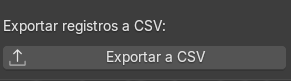
\includegraphics[width=0.65\textwidth]{diagramas/exportacion.png}
    \caption{Botón de exportación del CSV generado por el Data Logger 3D.}
    \label{fig:e-export-csv-logger}
\end{figure}

\begin{figure}[H]
    \centering
    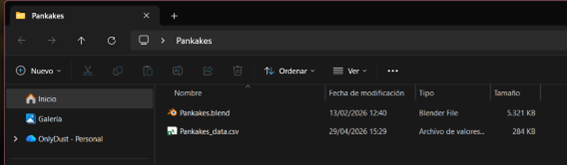
\includegraphics[width=0.85\textwidth]{diagramas/pankakes.png}
    \caption{Archivo CSV exportado en la misma carpeta que el proyecto de Blender.}
    \label{fig:e-csv-exportado}
\end{figure}


\section{Uso del add-on de análisis}
\label{sec:e-uso-analisis}

\begin{figure}[H]
    \centering
    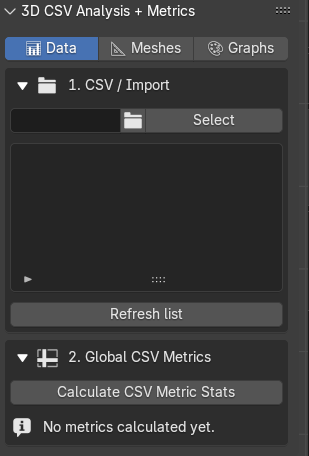
\includegraphics[width=0.75\textwidth]{diagramas/analisisinicial.png}
    \caption{Pestaña de análisis CSV del add-on de análisis y visualización.}
    \label{fig:e-panel-analisis-csv}
\end{figure}

\begin{figure}[H]
    \centering
    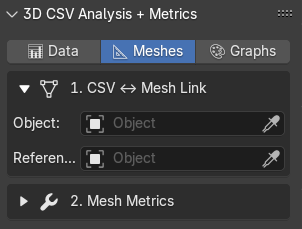
\includegraphics[width=0.75\textwidth]{diagramas/mallas.png}
    \caption{Pestaña de métricas de malla del add-on de análisis y visualización.}
    \label{fig:e-panel-metricas-malla}
\end{figure}

\begin{figure}[H]
    \centering
    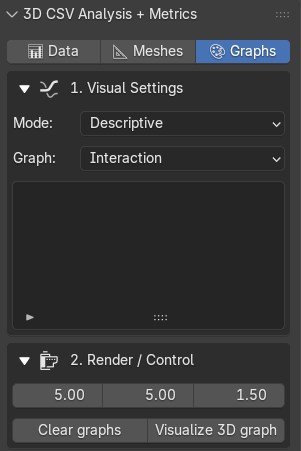
\includegraphics[width=0.75\textwidth]{diagramas/graficos.png}
    \caption{Pestaña de gráficos y visualizaciones del add-on de análisis y visualización.}
    \label{fig:e-panel-graficos-visualizaciones}
\end{figure}

\subsection{Selección de CSV o carpeta}
\label{subsec:e-seleccion-csv}

El add-on de análisis permite seleccionar un CSV individual o una carpeta con varios CSV. La selección de carpeta resulta útil cuando se desea comparar sesiones o usuarios. Los archivos deben conservar la estructura de cabecera generada por el logger.

\begin{enumerate}
    \item Abrir el panel del add-on de análisis en Blender.
    \item Seleccionar el CSV exportado o la carpeta que contiene varios CSV.
    \item Comprobar que la ruta aparece correctamente en el panel.
    \item Ejecutar la acción de cálculo correspondiente.
\end{enumerate}

\begin{figure}[H]
    \centering
    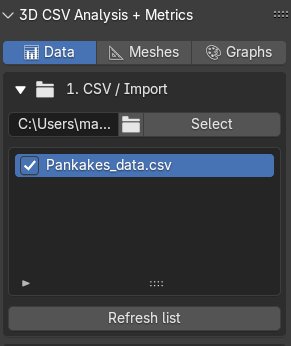
\includegraphics[width=0.85\textwidth]{diagramas/csv1.png}
    \caption{Selección de un archivo CSV generado por el Data Logger 3D.}
    \label{fig:e-seleccion-csv}
\end{figure}

\begin{figure}[H]
    \centering
    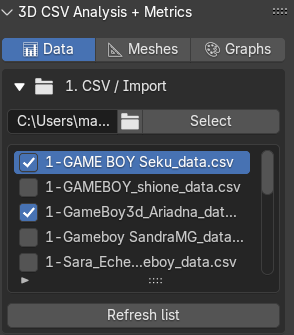
\includegraphics[width=0.85\textwidth]{diagramas/csv2.png}
    \caption{Selección de una carpeta con varios CSV para análisis comparativo.}
    \label{fig:e-seleccion-carpeta-csv}
\end{figure}

\subsection{Cálculo de métricas estadísticas}
\label{subsec:e-calculo-a1-a17}

El cálculo de métricas estadísticas procesa los registros CSV y genera indicadores A1--A17. Estas métricas resumen duración, pausas, velocidad, proximidad, manipulación de vista, actividad, evolución de vértices, errores, trabajo UV y cambios de objeto. La interfaz muestra resultados agrupados para evitar repetición.

\begin{figure}[H]
    \centering
    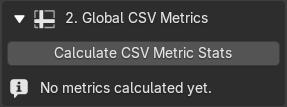
\includegraphics[width=0.75\textwidth]{diagramas/boton_metricas.png}
    \caption{Acción de cálculo de métricas estadísticas a partir del CSV seleccionado.}
    \label{fig:e-boton-calculo-metricas}
\end{figure}

\begin{table}[H]
\centering
\scriptsize
\renewcommand{\arraystretch}{1.12}
\begin{tabularx}{\textwidth}{p{3cm}X}
\toprule
\textbf{Bloque visible} & \textbf{Interpretación práctica} \\
\midrule
A1 & Duración total de la sesión. \\
A2--A3 & Pausas y distribución temporal de pausas. \\
A4--A5 & Velocidad de movimiento y proximidad al objeto. \\
A6--A9 & Manipulación de vista, velocidad en actividad/inactividad y distancia recorrida. \\
A10--A11 & Estrategias de aceleración o cambios de ritmo. \\
A12--A13 & Evolución de vértices y errores topológicos. \\
A14--A17 & Trabajo en \textit{Object Mode}, UV, evolución de malla y cambios de objeto. \\
\bottomrule
\end{tabularx}
\caption{Lectura práctica de los bloques A1--A17.}
\label{tab:e-interpretacion-a}
\end{table}

Faltan las capturas reales de las propias metricas, se meteran cuando el código este acabado.
%\begin{figure}[H]
%    \centering
%    \includegraphics[width=0.8\textwidth]{diagramas/e17_resultados_a1_a17.png}
%    \caption{Resultados de las métricas estadísticas A1--A17 mostrados en bloques compactos.}
%    \label{fig:e-resultados-a1-a17}
%end{figure}


\subsection{Cálculo de métricas geométricas y UV}
\label{subsec:e-calculo-geom-uv}

Para calcular métricas geométricas o UV se debe seleccionar el objeto de Blender correspondiente. Algunas métricas pueden requerir además un objeto de referencia, por ejemplo en comparaciones de similitud o en el cálculo de la distancia de Hausdorff. Si la malla no tiene UV, el sistema no podrá calcular métricas de área, islas, estiramiento o densidad de texeles.

En el caso de la métrica de similitud, es importante que el objeto analizado y el objeto de referencia se encuentren lo más alineados posible antes de realizar el cálculo. Para obtener una comparación más precisa, ambos modelos deberían presentar una orientación, escala y posición similares. Este ajuste debe realizarse manualmente en Blender, ya que la alineación automática entre modelos puede resultar compleja y no siempre fiable, especialmente cuando existen diferencias de escala, rotación, topología o nivel de detalle entre los objetos comparados.

Por tanto, antes de ejecutar la comparación de similitud, se recomienda revisar visualmente ambos objetos y, si es necesario, ajustar manualmente su rotación, tamaño y colocación en la escena. De esta forma, la métrica refleja con mayor fidelidad las diferencias geométricas reales entre los modelos, en lugar de verse afectada por desplazamientos, escalados o rotaciones previas.

Las métricas geométricas ayudan a valorar la calidad de la malla: caras no cuadrangulares, duplicados de vértices, normales potencialmente invertidas, ángulos, similitud y distancia respecto a una referencia. Las métricas UV ayudan a revisar el despliegue y la consistencia de coordenadas UV.

\begin{quote}
\textbf{Nota:} para que la métrica de similitud sea más precisa, los objetos comparados deben estar previamente alineados de forma manual en cuanto a rotación, escala y posición. La herramienta no realiza una alineación automática completa, ya que este proceso puede ser ambiguo y difícil de generalizar para modelos con geometrías distintas.
\end{quote}

\begin{figure}[H]
    \centering
    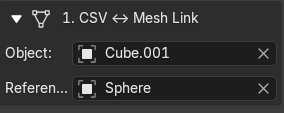
\includegraphics[width=0.8\textwidth]{diagramas/reference.png}
    \caption{Selección del objeto activo y el de referencia para el cálculo de métricas geométricas y UV.}
    \label{fig:e-objeto-activo-metricas}
\end{figure}

\begin{figure}[H]
    \centering
    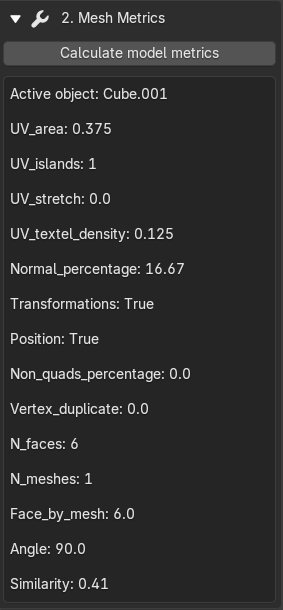
\includegraphics[width=0.8\textwidth]{diagramas/mesh_metrics.png}
    \caption{Resultados de métricas UV y geométricas calculadas sobre el objeto seleccionado.}
    \label{fig:e-resultados-geometricos}
\end{figure}

\subsection{Visualizaciones}
\label{subsec:e-visualizaciones}

El add-on puede generar visualizaciones dentro de Blender, como gráficos temporales, comparaciones entre CSV, superficies, radar o representaciones 3D. Antes de crear una nueva visualización se recomienda eliminar gráficos anteriores si el panel ofrece esa opción, para evitar acumulación de objetos en la escena.

\begin{figure}[H]
    \centering
    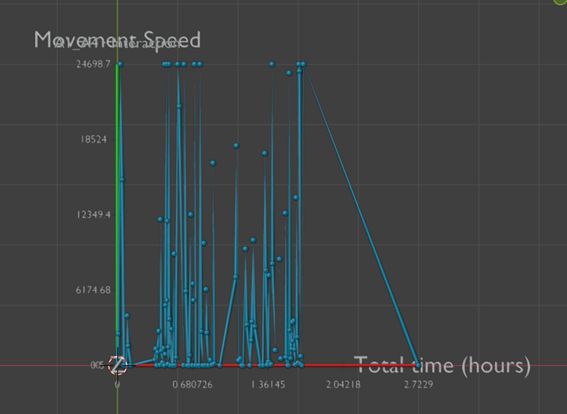
\includegraphics[width=0.9\textwidth]{diagramas/grafico1.png}
    \caption{Visualización temporal generada a partir de los datos de una sesión.}
    \label{fig:e-grafico-temporal}
\end{figure}

\begin{figure}[H]
    \centering
    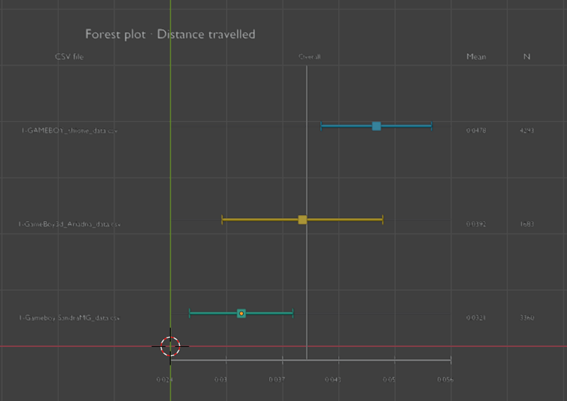
\includegraphics[width=0.9\textwidth]{diagramas/grafico2.png}
    \caption{Comparación visual de varias sesiones a partir de múltiples archivos CSV.}
    \label{fig:e-comparacion-multicsv}
\end{figure}

\begin{figure}[H]
    \centering
    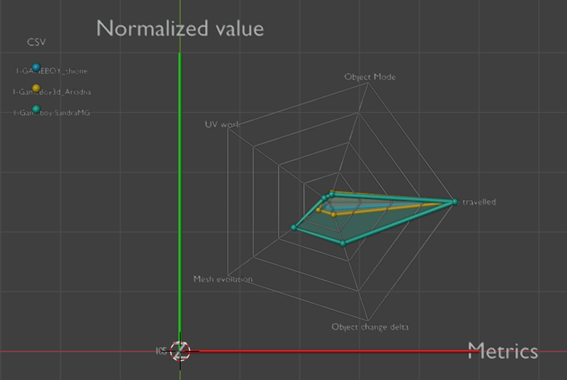
\includegraphics[width=0.9\textwidth]{diagramas/grafico3.png}
    \caption{Gráfico radar generado para representar métricas normalizadas de una sesión.}
    \label{fig:e-grafico-radar}
\end{figure}

\section{Interpretación de métricas}
\label{sec:e-interpretacion-metricas}

La interpretación debe realizarse con cautela. Una métrica alta no implica necesariamente un error: puede reflejar una sesión larga, una fase intensa de edición o una estrategia de trabajo concreta. Por ello, se recomienda analizar los bloques en conjunto y comparar sesiones con condiciones similares.

Las métricas temporales ayudan a identificar duración y pausas. Las métricas espaciales describen navegación y proximidad. Las métricas de estrategia reflejan cambios de modo, edición, UV y evolución de la malla. Las métricas geométricas y UV deben interpretarse junto con el estado visual del objeto, ya que dependen de la geometría seleccionada y de la existencia de referencia cuando proceda.

\section{Diagnóstico y resolución de incidencias}
\label{sec:e-diagnostico}

\begin{table}[H]
\centering
\scriptsize
\renewcommand{\arraystretch}{1.15}
\begin{tabularx}{\textwidth}{p{4cm}X X}
\toprule
\textbf{Incidencia} & \textbf{Causa probable} & \textbf{Solución recomendada} \\
\midrule
El logger no se inicia & Auto Run desactivado o add-on no activado. & Revisar preferencias, activar Auto Run si procede y comprobar que el add-on está habilitado. \\
No aparece el panel & Add-on no instalado o pestaña lateral cerrada. & Activar el add-on y abrir la barra lateral con la tecla \texttt{N}. \\
No se exporta CSV & El \texttt{.blend} no está guardado o no existe registro incrustado. & Guardar el proyecto, iniciar/detener captura y volver a exportar. \\
El CSV está vacío & No se detectaron cambios o la captura no llegó a iniciarse. & Repetir sesión comprobando el estado del logger. \\
El análisis rechaza datos & Cabecera incorrecta, valores no numéricos, NaN o infinitos. & Revisar el CSV y comprobar que procede del logger. \\
No se calculan métricas UV & El objeto no tiene capa UV activa. & Crear o seleccionar una capa UV válida. \\
La comparación geométrica falla & Falta objeto de referencia o la malla no es válida. & Seleccionar referencia y objeto objetivo correctamente. \\
La escena contiene demasiados gráficos & Visualizaciones anteriores no eliminadas. & Usar la opción de limpieza o borrar objetos generados. \\
\bottomrule
\end{tabularx}
\caption{Problemas frecuentes y soluciones recomendadas.}
\label{tab:e-incidencias}
\end{table}

\section{Consideraciones éticas y privacidad}
\label{sec:e-privacidad}

El uso del logger debe estar precedido por consentimiento informado. El sistema registra datos técnicos de interacción y modelado, no contenido personal directo. Aun así, se recomienda tratar los CSV como datos de investigación: almacenarlos en ubicaciones controladas, evitar compartirlos sin autorización y seudonimizar cualquier información que pueda asociarse a personas concretas.

Cuando los datos se utilicen en contexto académico, debe indicarse la finalidad del análisis, el tipo de datos capturados, la forma de almacenamiento y las condiciones de eliminación o reutilización. Si se incorporan participantes externos, deben añadirse los documentos de información y consentimiento correspondientes.

\section{Recomendaciones para análisis de datos}
\label{sec:e-recomendaciones}

Para obtener resultados comparables se recomienda utilizar nombres de archivo claros, conservar una carpeta por sesión o participante, no mezclar CSV generados con versiones incompatibles del logger y anotar manualmente cualquier incidencia relevante de la sesión. En comparaciones entre usuarios, las sesiones deberían tener condiciones similares de duración, tarea y versión de Blender.

También se recomienda revisar visualmente los modelos antes de interpretar métricas geométricas y UV. La comparación frente a un objeto de referencia solo es significativa si ambos modelos responden a una misma tarea o a una referencia común.

\section{Resumen operativo}
\label{sec:e-resumen-operativo}

El flujo básico de uso es el siguiente: instalar ambos add-ons, activar el logger, aceptar el consentimiento, iniciar captura, realizar la sesión de modelado, detener captura, exportar CSV, abrir el add-on de análisis, seleccionar CSV o carpeta, calcular métricas y revisar resultados. Este flujo separa captura y análisis, reduce interferencias durante el modelado y facilita la reutilización posterior de los registros.
